\chapter{Robert le Diable}

The pretext of an opera engagement was so much the more feasible, as
there chanced to be on that very night a more than ordinary attraction
at the Académie Royale. Levasseur, who had been suffering under severe
illness, made his reappearance in the character of \textit{Bertram}, and, as
usual, the announcement of the most admired production of the favorite
composer of the day had attracted a brilliant and fashionable audience.
Morcerf, like most other young men of rank and fortune, had his
orchestra stall, with the certainty of always finding a seat in at
least a dozen of the principal boxes occupied by persons of his
acquaintance; he had, moreover, his right of entry into the omnibus
box. Château-Renaud rented a stall beside his own, while Beauchamp, as
a journalist, had unlimited range all over the theatre. It happened
that on this particular night the minister’s box was placed at the
disposal of Lucien Debray, who offered it to the Comte de Morcerf, who
again, upon his rejection of it by Mercédès, sent it to Danglars, with
an intimation that he should probably do himself the honor of joining
the baroness and her daughter during the evening, in the event of their
accepting the box in question. The ladies received the offer with too
much pleasure to dream of a refusal. To no class of persons is the
presentation of a gratuitous opera-box more acceptable than to the
wealthy millionaire, who still hugs economy while boasting of carrying
a king’s ransom in his waistcoat pocket.

Danglars had, however, protested against showing himself in a
ministerial box, declaring that his political principles, and his
parliamentary position as member of the opposition party would not
permit him so to commit himself; the baroness had, therefore,
despatched a note to Lucien Debray, bidding him call for them, it being
wholly impossible for her to go alone with Eugénie to the opera.

There is no gainsaying the fact that a very unfavorable construction
would have been put upon the circumstance if the two women had gone
without escort, while the addition of a third, in the person of her
mother’s admitted lover, enabled Mademoiselle Danglars to defy malice
and ill-nature. One must take the world as one finds it.

\begin{figure}[ht]
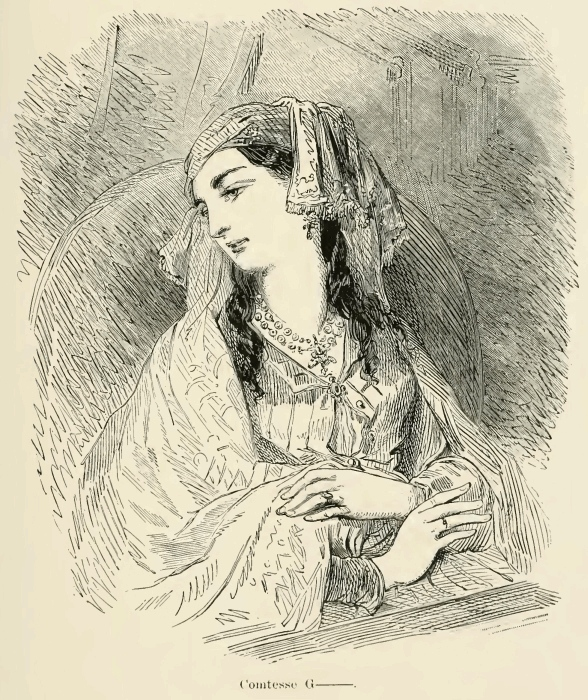
\includegraphics[width=\textwidth]{30083m.jpg}
\end{figure}

The curtain rose, as usual, to an almost empty house, it being one of
the absurdities of Parisian fashion never to appear at the opera until
after the beginning of the performance, so that the first act is
generally played without the slightest attention being paid to it, that
part of the audience already assembled being too much occupied in
observing the fresh arrivals, while nothing is heard but the noise of
opening and shutting doors, and the buzz of conversation.

“Surely,” said Albert, as the door of a box on the first circle opened,
“that must be the Countess G——.”

“And who is the Countess G——?” inquired Château-Renaud.

“What a question! Now, do you know, baron, I have a great mind to pick
a quarrel with you for asking it; as if all the world did not know who
the Countess G—— was.”

“Ah, to be sure,” replied Château-Renaud; “the lovely Venetian, is it
not?”

“Herself.” At this moment the countess perceived Albert, and returned
his salutation with a smile.

“You know her, it seems?” said Château-Renaud.

“Franz introduced me to her at Rome,” replied Albert.

“Well, then, will you do as much for me in Paris as Franz did for you
in Rome?”

“With pleasure.”

There was a cry of “Shut up!” from the audience. This manifestation on
the part of the spectators of their wish to be allowed to hear the
music, produced not the slightest effect on the two young men, who
continued their conversation.

“The countess was present at the races in the Champ-de-Mars,” said
Château-Renaud.

“Today?”

“Yes.”

“Bless me, I quite forgot the races. Did you bet?”

“Oh, merely a paltry fifty louis.”

“And who was the winner?”

“Nautilus. I staked on him.”

“But there were three races, were there not?”

“Yes; there was the prize given by the Jockey Club—a gold cup, you
know—and a very singular circumstance occurred about that race.”

“What was it?”

“Oh, shut up!” again interposed some of the audience.

“Why, it was won by a horse and rider utterly unknown on the course.”

“Is that possible?”

“True as day. The fact was, nobody had observed a horse entered by the
name of Vampa, or that of a jockey styled Job, when, at the last
moment, a splendid roan, mounted by a jockey about as big as your fist,
presented themselves at the starting-post. They were obliged to stuff
at least twenty pounds weight of shot in the small rider’s pockets, to
make him weight; but with all that he outstripped Ariel and Barbare,
against whom he ran, by at least three whole lengths.”

“And was it not found out at last to whom the horse and jockey
belonged?”

“No.”

“You say that the horse was entered under the name of Vampa?”

“Exactly; that was the title.”

“Then,” answered Albert, “I am better informed than you are, and know
who the owner of that horse was.”

“Shut up, there!” cried the pit in chorus. And this time the tone and
manner in which the command was given, betokened such growing hostility
that the two young men perceived, for the first time, that the mandate
was addressed to them. Leisurely turning round, they calmly scrutinized
the various countenances around them, as though demanding some one
person who would take upon himself the responsibility of what they
deemed excessive impertinence; but as no one responded to the
challenge, the friends turned again to the front of the theatre, and
affected to busy themselves with the stage. At this moment the door of
the minister’s box opened, and Madame Danglars, accompanied by her
daughter, entered, escorted by Lucien Debray, who assiduously conducted
them to their seats.

“Ha, ha,” said Château-Renaud, “here come some friends of yours,
viscount! What are you looking at there? don’t you see they are trying
to catch your eye?”

Albert turned round, just in time to receive a gracious wave of the fan
from the baroness; as for Mademoiselle Eugénie, she scarcely vouchsafed
to waste the glances of her large black eyes even upon the business of
the stage.

“I tell you what, my dear fellow,” said Château-Renaud, “I cannot
imagine what objection you can possibly have to Mademoiselle
Danglars—that is, setting aside her want of ancestry and somewhat
inferior rank, which by the way I don’t think you care very much about.
Now, barring all that, I mean to say she is a deuced fine girl!”

“Handsome, certainly,” replied Albert, “but not to my taste, which I
confess, inclines to something softer, gentler, and more feminine.”

“Ah, well,” exclaimed Château-Renaud, who because he had seen his
thirtieth summer fancied himself duly warranted in assuming a sort of
paternal air with his more youthful friend, “you young people are never
satisfied; why, what would you have more? your parents have chosen you
a bride built on the model of Diana, the huntress, and yet you are not
content.”

“No, for that very resemblance affrights me; I should have liked
something more in the manner of the Venus of Milo or Capua; but this
chase-loving Diana, continually surrounded by her nymphs, gives me a
sort of alarm lest she should some day bring on me the fate of Actæon.”

And, indeed, it required but one glance at Mademoiselle Danglars to
comprehend the justness of Morcerf’s remark. She was beautiful, but her
beauty was of too marked and decided a character to please a fastidious
taste; her hair was raven black, but its natural waves seemed somewhat
rebellious; her eyes, of the same color as her hair, were surmounted by
well-arched brows, whose great defect, however, consisted in an almost
habitual frown, while her whole physiognomy wore that expression of
firmness and decision so little in accordance with the gentler
attributes of her sex—her nose was precisely what a sculptor would have
chosen for a chiselled Juno. Her mouth, which might have been found
fault with as too large, displayed teeth of pearly whiteness, rendered
still more conspicuous by the brilliant carmine of her lips,
contrasting vividly with her naturally pale complexion. But that which
completed the almost masculine look Morcerf found so little to his
taste, was a dark mole, of much larger dimensions than these freaks of
nature generally are, placed just at the corner of her mouth; and the
effect tended to increase the expression of self-dependence that
characterized her countenance.

The rest of Mademoiselle Eugénie’s person was in perfect keeping with
the head just described; she, indeed, reminded one of Diana, as
Château-Renaud observed, but her bearing was more haughty and resolute.

As regarded her attainments, the only fault to be found with them was
the same that a fastidious connoisseur might have found with her
beauty, that they were somewhat too erudite and masculine for so young
a person. She was a perfect linguist, a first-rate artist, wrote
poetry, and composed music; to the study of the latter she professed to
be entirely devoted, following it with an indefatigable perseverance,
assisted by a schoolfellow,—a young woman without fortune whose talent
promised to develop into remarkable powers as a singer. It was rumored
that she was an object of almost paternal interest to one of the
principal composers of the day, who excited her to spare no pains in
the cultivation of her voice, which might hereafter prove a source of
wealth and independence. But this counsel effectually decided
Mademoiselle Danglars never to commit herself by being seen in public
with one destined for a theatrical life; and acting upon this
principle, the banker’s daughter, though perfectly willing to allow
Mademoiselle Louise d’Armilly (that was the name of the young virtuosa)
to practice with her through the day, took especial care not to be seen
in her company. Still, though not actually received at the Hôtel
Danglars in the light of an acknowledged friend, Louise was treated
with far more kindness and consideration than is usually bestowed on a
governess.

The curtain fell almost immediately after the entrance of Madame
Danglars into her box, the band quitted the orchestra for the
accustomed half-hour’s interval allowed between the acts, and the
audience were left at liberty to promenade the salon or lobbies, or to
pay and receive visits in their respective boxes.

Morcerf and Château-Renaud were amongst the first to avail themselves
of this permission. For an instant the idea struck Madame Danglars that
this eagerness on the part of the young viscount arose from his
impatience to join her party, and she whispered her expectations to her
daughter, that Albert was hurrying to pay his respects to them.
Mademoiselle Eugénie, however, merely returned a dissenting movement of
the head, while, with a cold smile, she directed the attention of her
mother to an opposite box on the first circle, in which sat the
Countess G——, and where Morcerf had just made his appearance.

\begin{figure}[ht]
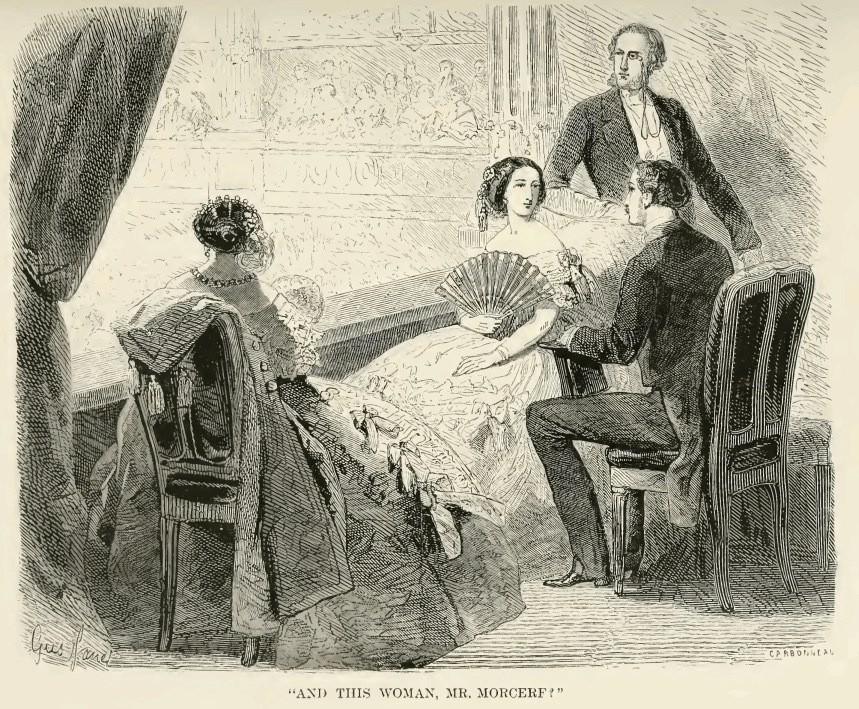
\includegraphics[width=\textwidth]{30087m.jpg}
\end{figure}

“So we meet again, my travelling friend, do we?” cried the countess,
extending her hand to him with all the warmth and cordiality of an old
acquaintance; “it was really very good of you to recognize me so
quickly, and still more so to bestow your first visit on me.”

“Be assured,” replied Albert, “that if I had been aware of your arrival
in Paris, and had known your address, I should have paid my respects to
you before this. Allow me to introduce my friend, Baron de
Château-Renaud, one of the few true gentlemen now to be found in
France, and from whom I have just learned that you were a spectator of
the races in the Champ-de-Mars, yesterday.”

Château-Renaud bowed to the countess.

“So you were at the races, baron?” inquired the countess eagerly.

“Yes, madame.”

“Well, then,” pursued Madame G—— with considerable animation, “you can
probably tell me who won the Jockey Club stakes?”

“I am sorry to say I cannot,” replied the baron; “and I was just asking
the same question of Albert.”

“Are you very anxious to know, countess?” asked Albert.

“To know what?”

“The name of the owner of the winning horse?”

“Excessively; only imagine—but do tell me, viscount, whether you really
are acquainted with it or no?”

“I beg your pardon, madame, but you were about to relate some story,
were you not? You said, ‘only imagine,’—and then paused. Pray
continue.”

“Well, then, listen. You must know I felt so interested in the splendid
roan horse, with his elegant little rider, so tastefully dressed in a
pink satin jacket and cap, that I could not help praying for their
success with as much earnestness as though the half of my fortune were
at stake; and when I saw them outstrip all the others, and come to the
winning-post in such gallant style, I actually clapped my hands with
joy. Imagine my surprise, when, upon returning home, the first object I
met on the staircase was the identical jockey in the pink jacket! I
concluded that, by some singular chance, the owner of the winning horse
must live in the same hotel as myself; but, as I entered my apartments,
I beheld the very gold cup awarded as a prize to the unknown horse and
rider. Inside the cup was a small piece of paper, on which were written
these words—‘From Lord Ruthven to Countess G——.’”

“Precisely; I was sure of it,” said Morcerf.

“Sure of what?”

“That the owner of the horse was Lord Ruthven himself.”

“What Lord Ruthven do you mean?”

“Why, our Lord Ruthven—the Vampire of the Salle Argentina!”

“Is it possible?” exclaimed the countess; “is he here in Paris?”

“To be sure,—why not?”

“And you visit him?—meet him at your own house and elsewhere?”

“I assure you he is my most intimate friend, and M. de Château-Renaud
has also the honor of his acquaintance.”

“But why are you so sure of his being the winner of the Jockey Club
prize?”

“Was not the winning horse entered by the name of Vampa?”

“What of that?”

“Why, do you not recollect the name of the celebrated bandit by whom I
was made prisoner?”

“Oh, yes.”

“And from whose hands the count extricated me in so wonderful a
manner?”

“To be sure, I remember it all now.”

“He called himself Vampa. You see, it’s evident where the count got the
name.”

“But what could have been his motive for sending the cup to me?”

“In the first place, because I had spoken much of you to him, as you
may believe; and in the second, because he delighted to see a
countrywoman take so lively an interest in his success.”

“I trust and hope you never repeated to the count all the foolish
remarks we used to make about him?”

“I should not like to affirm upon oath that I have not. Besides, his
presenting you the cup under the name of Lord Ruthven——”

“Oh, but that is dreadful! Why, the man must owe me a fearful grudge.”

“Does his action appear like that of an enemy?”

“No; certainly not.”

“Well, then——”

“And so he is in Paris?”

“Yes.”

“And what effect does he produce?”

“Why,” said Albert, “he was talked about for a week; then the
coronation of the queen of England took place, followed by the theft of
Mademoiselle Mars’s diamonds; and so people talked of something else.”

“My good fellow,” said Château-Renaud, “the count is your friend and
you treat him accordingly. Do not believe what Albert is telling you,
countess; so far from the sensation excited in the Parisian circles by
the appearance of the Count of Monte Cristo having abated, I take upon
myself to declare that it is as strong as ever. His first astounding
act upon coming amongst us was to present a pair of horses, worth
32,000 francs, to Madame Danglars; his second, the almost miraculous
preservation of Madame de Villefort’s life; now it seems that he has
carried off the prize awarded by the Jockey Club. I therefore maintain,
in spite of Morcerf, that not only is the count the object of interest
at this present moment, but also that he will continue to be so for a
month longer if he pleases to exhibit an eccentricity of conduct which,
after all, may be his ordinary mode of existence.”

“Perhaps you are right,” said Morcerf; “meanwhile, who is in the
Russian ambassador’s box?”

“Which box do you mean?” asked the countess.

“The one between the pillars on the first tier—it seems to have been
fitted up entirely afresh.”

“Did you observe anyone during the first act?” asked Château-Renaud.

“Where?”

“In that box.”

“No,” replied the countess, “it was certainly empty during the first
act;” then, resuming the subject of their previous conversation, she
said, “And so you really believe it was your mysterious Count of Monte
Cristo that gained the prize?”

“I am sure of it.”

“And who afterwards sent the cup to me?”

“Undoubtedly.”

“But I don’t know him,” said the countess; “I have a great mind to
return it.”

“Do no such thing, I beg of you; he would only send you another, formed
of a magnificent sapphire, or hollowed out of a gigantic ruby. It is
his way, and you must take him as you find him.”

At this moment the bell rang to announce the drawing up of the curtain
for the second act. Albert rose to return to his place.

“Shall I see you again?” asked the countess.

“At the end of the next act, with your permission, I will come and
inquire whether there is anything I can do for you in Paris?”

“Pray take notice,” said the countess, “that my present residence is 22
Rue de Rivoli, and that I am at home to my friends every Saturday
evening. So now, you are both forewarned.”

The young men bowed, and quitted the box. Upon reaching their stalls,
they found the whole of the audience in the parterre standing up and
directing their gaze towards the box formerly possessed by the Russian
ambassador. A man of from thirty-five to forty years of age, dressed in
deep black, had just entered, accompanied by a young woman dressed
after the Eastern style. The lady was surpassingly beautiful, while the
rich magnificence of her attire drew all eyes upon her.

“Hullo,” said Albert; “it is Monte Cristo and his Greek!”

The strangers were, indeed, no other than the count and Haydée. In a
few moments the young girl had attracted the attention of the whole
house, and even the occupants of the boxes leaned forward to scrutinize
her magnificent diamonds.

The second act passed away during one continued buzz of voices—one deep
whisper—intimating that some great and universally interesting event
had occurred; all eyes, all thoughts, were occupied with the young and
beautiful woman, whose gorgeous apparel and splendid jewels made a most
extraordinary spectacle.

Upon this occasion an unmistakable sign from Madame Danglars intimated
her desire to see Albert in her box directly the curtain fell on the
second act, and neither the politeness nor good taste of Morcerf would
permit his neglecting an invitation so unequivocally given. At the
close of the act he therefore went to the baroness.

Having bowed to the two ladies, he extended his hand to Debray. By the
baroness he was most graciously welcomed, while Eugénie received him
with her accustomed coldness.

“My dear fellow,” said Debray, “you have come in the nick of time.
There is madame overwhelming me with questions respecting the count;
she insists upon it that I can tell her his birth, education, and
parentage, where he came from, and whither he is going. Being no
disciple of Cagliostro, I was wholly unable to do this; so, by way of
getting out of the scrape, I said, ‘Ask Morcerf; he has got the whole
history of his beloved Monte Cristo at his fingers’ ends;’ whereupon
the baroness signified her desire to see you.”

“Is it not almost incredible,” said Madame Danglars, “that a person
having at least half a million of secret-service money at his command,
should possess so little information?”

“Let me assure you, madame,” said Lucien, “that had I really the sum
you mention at my disposal, I would employ it more profitably than in
troubling myself to obtain particulars respecting the Count of Monte
Cristo, whose only merit in my eyes consists in his being twice as rich
as a nabob. However, I have turned the business over to Morcerf, so
pray settle it with him as may be most agreeable to you; for my own
part, I care nothing about the count or his mysterious doings.”

\begin{figure}[ht]
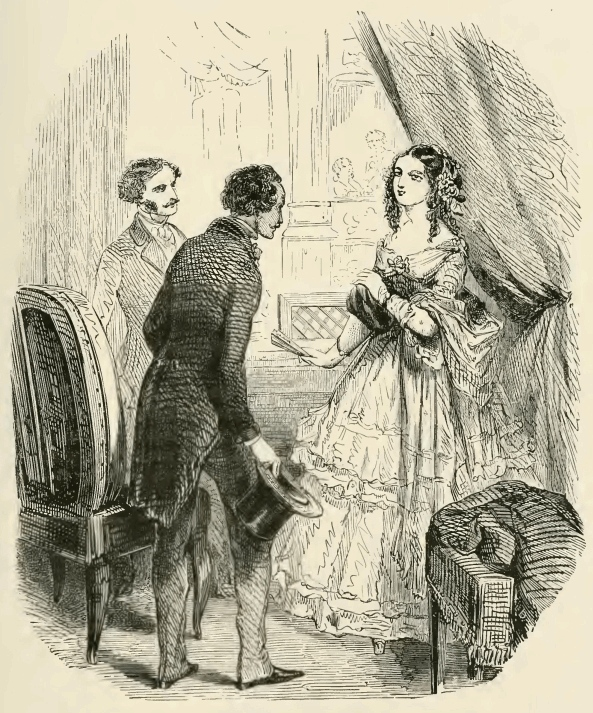
\includegraphics[width=\textwidth]{30093m.jpg}
\end{figure}

“I am very sure no nabob would have sent me a pair of horses worth
32,000 francs, wearing on their heads four diamonds valued at 5,000
francs each.”

“He seems to have a mania for diamonds,” said Morcerf, smiling, “and I
verily believe that, like Potemkin, he keeps his pockets filled, for
the sake of strewing them along the road, as Tom Thumb did his flint
stones.”

“Perhaps he has discovered some mine,” said Madame Danglars. “I suppose
you know he has an order for unlimited credit on the baron’s banking
establishment?”

“I was not aware of it,” replied Albert, “but I can readily believe
it.”

“And, further, that he stated to M. Danglars his intention of only
staying a year in Paris, during which time he proposed to spend six
millions.

“He must be the Shah of Persia, travelling \textit{incog}.”

“Have you noticed the remarkable beauty of the young woman, M. Lucien?”
inquired Eugénie.

“I really never met with one woman so ready to do justice to the charms
of another as yourself,” responded Lucien, raising his lorgnette to his
eye. “A most lovely creature, upon my soul!” was his verdict.

“Who is this young person, M. de Morcerf?” inquired Eugénie; “does
anybody know?”

“Mademoiselle,” said Albert, replying to this direct appeal, “I can
give you very exact information on that subject, as well as on most
points relative to the mysterious person of whom we are now
conversing—the young woman is a Greek.”

“So I should suppose by her dress; if you know no more than that,
everyone here is as well-informed as yourself.”

“I am extremely sorry you find me so ignorant a \textit{cicerone},” replied
Morcerf, “but I am reluctantly obliged to confess, I have nothing
further to communicate—yes, stay, I do know one thing more, namely,
that she is a musician, for one day when I chanced to be breakfasting
with the count, I heard the sound of a guzla—it is impossible that it
could have been touched by any other finger than her own.”

“Then your count entertains visitors, does he?” asked Madame Danglars.

“Indeed he does, and in a most lavish manner, I can assure you.”

“I must try and persuade M. Danglars to invite him to a ball or dinner,
or something of the sort, that he may be compelled to ask us in
return.”

“What,” said Debray, laughing; “do you really mean you would go to his
house?”

“Why not? my husband could accompany me.”

“But do you know this mysterious count is a bachelor?”

“You have ample proof to the contrary, if you look opposite,” said the
baroness, as she laughingly pointed to the beautiful Greek.

“No, no!” exclaimed Debray; “that girl is not his wife: he told us
himself she was his slave. Do you not recollect, Morcerf, his telling
us so at your breakfast?”

“Well, then,” said the baroness, “if slave she be, she has all the air
and manner of a princess.”

“Of the ‘Arabian Nights’.”

“If you like; but tell me, my dear Lucien, what it is that constitutes
a princess. Why, diamonds—and she is covered with them.”

“To me she seems overloaded,” observed Eugénie; “she would look far
better if she wore fewer, and we should then be able to see her finely
formed throat and wrists.”

“See how the artist peeps out!” exclaimed Madame Danglars. “My poor
Eugénie, you must conceal your passion for the fine arts.”

“I admire all that is beautiful,” returned the young lady.

“What do you think of the count?” inquired Debray; “he is not much
amiss, according to my ideas of good looks.”

“The count,” repeated Eugénie, as though it had not occurred to her to
observe him sooner; “the count?—oh, he is so dreadfully pale.”

“I quite agree with you,” said Morcerf; “and the secret of that very
pallor is what we want to find out. The Countess G—— insists upon it
that he is a vampire.”

“Then the Countess G—— has returned to Paris, has she?” inquired the
baroness.

“Is that she, mamma?” asked Eugénie; “almost opposite to us, with that
profusion of beautiful light hair?”

“Yes,” said Madame Danglars, “that is she. Shall I tell you what you
ought to do, Morcerf?”

“Command me, madame.”

“Well, then, you should go and bring your Count of Monte Cristo to us.”

“What for?” asked Eugénie.

“What for? Why, to converse with him, of course. Have you really no
desire to meet him?”

“None whatever,” replied Eugénie.

“Strange child,” murmured the baroness.

“He will very probably come of his own accord,” said Morcerf. “There;
do you see, madame, he recognizes you, and bows.”

The baroness returned the salute in the most smiling and graceful
manner.

“Well,” said Morcerf, “I may as well be magnanimous, and tear myself
away to forward your wishes. Adieu; I will go and try if there are any
means of speaking to him.”

“Go straight to his box; that will be the simplest plan.”

“But I have never been presented.”

“Presented to whom?”

“To the beautiful Greek.”

“You say she is only a slave?”

“While you assert that she is a queen, or at least a princess. No; I
hope that when he sees me leave you, he will come out.”

“That is possible—go.”

“I am going,” said Albert, as he made his parting bow.

Just as he was passing the count’s box, the door opened, and Monte
Cristo came forth. After giving some directions to Ali, who stood in
the lobby, the count took Albert’s arm. Carefully closing the box door,
Ali placed himself before it, while a crowd of spectators assembled
round the Nubian.

“Upon my word,” said Monte Cristo, “Paris is a strange city, and the
Parisians a very singular people. See that cluster of persons collected
around poor Ali, who is as much astonished as themselves; really one
might suppose he was the only Nubian they had ever beheld. Now I can
promise you, that a Frenchman might show himself in public, either in
Tunis, Constantinople, Bagdad, or Cairo, without being treated in that
way.”

“That shows that the Eastern nations have too much good sense to waste
their time and attention on objects undeserving of either. However, as
far as Ali is concerned, I can assure you, the interest he excites is
merely from the circumstance of his being your attendant—you, who are
at this moment the most celebrated and fashionable person in Paris.”

“Really? and what has procured me so flattering a distinction?”

“What? why, yourself, to be sure! You give away horses worth a thousand
louis; you save the lives of ladies of high rank and beauty; under the
name of Major Black you run thoroughbreds ridden by tiny urchins not
larger than marmots; then, when you have carried off the golden trophy
of victory, instead of setting any value on it, you give it to the
first handsome woman you think of!”

“And who has filled your head with all this nonsense?”

“Why, in the first place, I heard it from Madame Danglars, who, by the
by, is dying to see you in her box, or to have you seen there by
others; secondly, I learned it from Beauchamp’s journal; and thirdly,
from my own imagination. Why, if you sought concealment, did you call
your horse Vampa?”

“That was an oversight, certainly,” replied the count; “but tell me,
does the Count of Morcerf never visit the Opera? I have been looking
for him, but without success.”

“He will be here tonight.”

“In what part of the house?”

“In the baroness’s box, I believe.”

“That charming young woman with her is her daughter?”

“Yes.”

“I congratulate you.”

Morcerf smiled.

“We will discuss that subject at length some future time,” said he.
“But what do you think of the music?”

“What music?”

“Why, the music you have been listening to.”

“Oh, it is well enough as the production of a human composer, sung by
featherless bipeds, to quote the late Diogenes.”

“From which it would seem, my dear count, that you can at pleasure
enjoy the seraphic strains that proceed from the seven choirs of
paradise?”

\begin{figure}[ht]
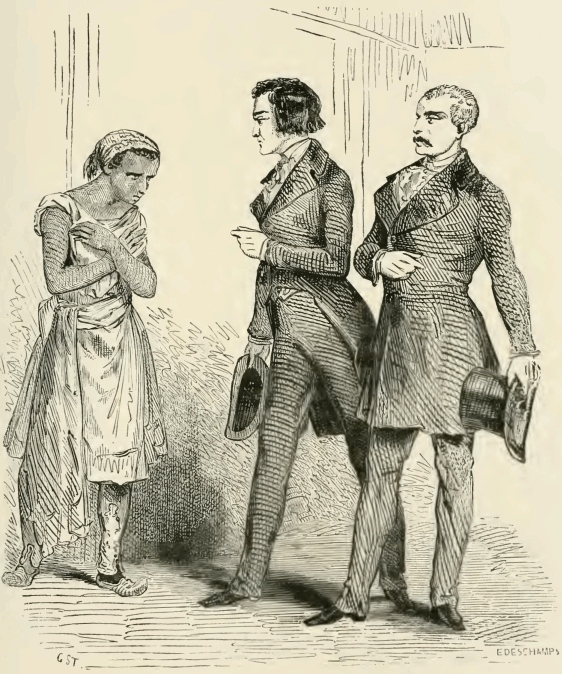
\includegraphics[width=\textwidth]{30097m.jpg}
\end{figure}

“You are right, in some degree; when I wish to listen to sounds more
exquisitely attuned to melody than mortal ear ever yet listened to, I
go to sleep.”

“Then sleep here, my dear count. The conditions are favorable; what
else was opera invented for?”

“No, thank you. Your orchestra is too noisy. To sleep after the manner
I speak of, absolute calm and silence are necessary, and then a certain
preparation——”

“I know—the famous hashish!”

“Precisely. So, my dear viscount, whenever you wish to be regaled with
music come and sup with me.”

“I have already enjoyed that treat when breakfasting with you,” said
Morcerf.

“Do you mean at Rome?”

“I do.”

“Ah, then, I suppose you heard Haydée’s guzla; the poor exile
frequently beguiles a weary hour in playing over to me the airs of her
native land.”

Morcerf did not pursue the subject, and Monte Cristo himself fell into
a silent reverie.

The bell rang at this moment for the rising of the curtain.

“You will excuse my leaving you,” said the count, turning in the
direction of his box.

“What? Are you going?”

“Pray, say everything that is kind to Countess G—— on the part of her
friend the vampire.”

“And what message shall I convey to the baroness!”

“That, with her permission, I shall do myself the honor of paying my
respects in the course of the evening.”

The third act had begun; and during its progress the Count of Morcerf,
according to his promise, made his appearance in the box of Madame
Danglars. The Count of Morcerf was not a person to excite either
interest or curiosity in a place of public amusement; his presence,
therefore, was wholly unnoticed, save by the occupants of the box in
which he had just seated himself.

The quick eye of Monte Cristo however, marked his coming; and a slight
though meaning smile passed over his lips. Haydée, whose soul seemed
centred in the business of the stage, like all unsophisticated natures,
delighted in whatever addressed itself to the eye or ear.

\begin{figure}[ht]
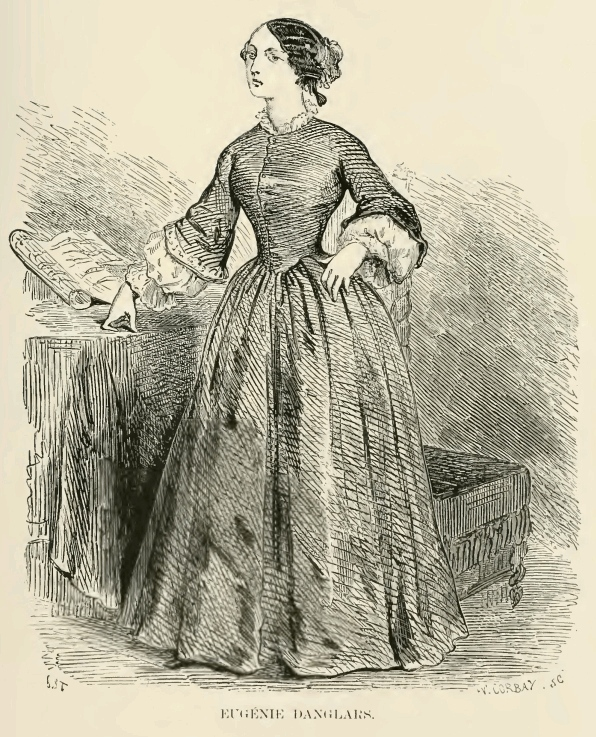
\includegraphics[width=\textwidth]{30099m.jpg}
\end{figure}

The third act passed off as usual. Mesdemoiselles Noblet, Julia, and
Leroux executed the customary pirouettes; Robert duly challenged the
Prince of Granada; and the royal father of the princess Isabella,
taking his daughter by the hand, swept round the stage with majestic
strides, the better to display the rich folds of his velvet robe and
mantle. After which the curtain again fell, and the spectators poured
forth from the theatre into the lobbies and salon.

The count left his box, and a moment later was saluting the Baronne
Danglars, who could not restrain a cry of mingled pleasure and
surprise.

“You are welcome, count!” she exclaimed, as he entered. “I have been
most anxious to see you, that I might repeat orally the thanks writing
can so ill express.”

“Surely so trifling a circumstance cannot deserve a place in your
remembrance. Believe me, madame, I had entirely forgotten it.”

“But it is not so easy to forget, monsieur, that the very next day
after your princely gift you saved the life of my dear friend, Madame
de Villefort, which was endangered by the very animals your generosity
restored to me.”

\begin{figure}[ht]
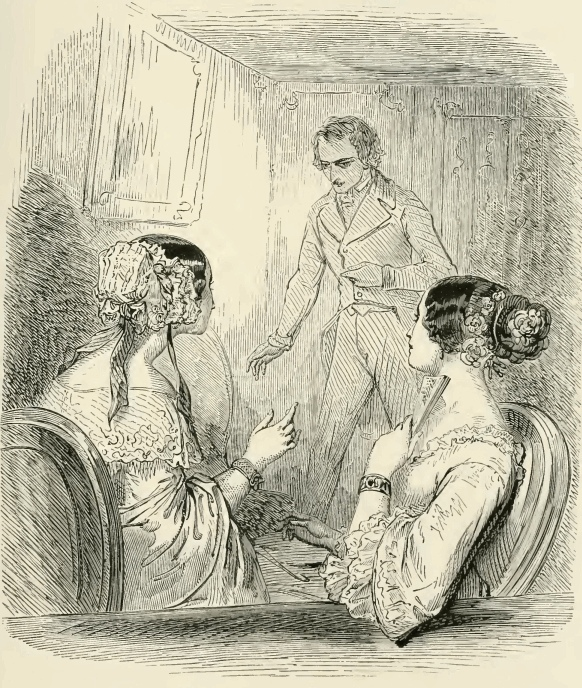
\includegraphics[width=\textwidth]{30101m.jpg}
\end{figure}

“This time, at least, I do not deserve your thanks. It was Ali, my
Nubian slave, who rendered this service to Madame de Villefort.”

“Was it Ali,” asked the Count of Morcerf, “who rescued my son from the
hands of bandits?”

“No, count,” replied Monte Cristo taking the hand held out to him by
the general; “in this instance I may fairly and freely accept your
thanks; but you have already tendered them, and fully discharged your
debt—if indeed there existed one—and I feel almost mortified to find
you still reverting to the subject. May I beg of you, baroness, to
honor me with an introduction to your daughter?”

“Oh, you are no stranger—at least not by name,” replied Madame
Danglars, “and the last two or three days we have really talked of
nothing but you. Eugénie,” continued the baroness, turning towards her
daughter, “this is the Count of Monte Cristo.”

The count bowed, while Mademoiselle Danglars bent her head slightly.

“You have a charming young person with you tonight, count,” said
Eugénie. “Is she your daughter?”

“No, mademoiselle,” said Monte Cristo, astonished at the coolness and
freedom of the question. “She is a poor unfortunate Greek left under my
care.”

“And what is her name?”

“Haydée,” replied Monte Cristo.

“A Greek?” murmured the Count of Morcerf.

“Yes, indeed, count,” said Madame Danglars; “and tell me, did you ever
see at the court of Ali Tepelini, whom you so gloriously and valiantly
served, a more exquisite beauty or richer costume?”

“Did I hear rightly, monsieur,” said Monte Cristo “that you served at
Yanina?”

“I was inspector-general of the pasha’s troops,” replied Morcerf; “and
it is no secret that I owe my fortune, such as it is, to the liberality
of the illustrious Albanese chief.”

“But look!” exclaimed Madame Danglars.

“Where?” stammered Morcerf.

“There,” said Monte Cristo placing his arms around the count, and
leaning with him over the front of the box, just as Haydée, whose eyes
were occupied in examining the theatre in search of her guardian,
perceived his pale features close to Morcerf’s face. It was as if the
young girl beheld the head of Medusa. She bent forwards as though to
assure herself of the reality of what she saw, then, uttering a faint
cry, threw herself back in her seat. The sound was heard by the people
about Ali, who instantly opened the box-door.

“Why, count,” exclaimed Eugénie, “what has happened to your ward? she
seems to have been taken suddenly ill.

“Very probably,” answered the count. “But do not be alarmed on her
account. Haydée’s nervous system is delicately organized, and she is
peculiarly susceptible to the odors even of flowers—nay, there are some
which cause her to faint if brought into her presence. However,”
continued Monte Cristo, drawing a small phial from his pocket, “I have
an infallible remedy.”

So saying, he bowed to the baroness and her daughter, exchanged a
parting shake of the hand with Debray and the count, and left Madame
Danglars’ box. Upon his return to Haydée he found her still very pale.
As soon as she saw him she seized his hand; her own hands were moist
and icy cold.

“Who was it you were talking with over there?” she asked.

“With the Count of Morcerf,” answered Monte Cristo. “He tells me he
served your illustrious father, and that he owes his fortune to him.”

“Wretch!” exclaimed Haydée, her eyes flashing with rage; “he sold my
father to the Turks, and the fortune he boasts of was the price of his
treachery! Did not you know that, my dear lord?”

“Something of this I heard in Epirus,” said Monte Cristo; “but the
particulars are still unknown to me. You shall relate them to me, my
child. They are, no doubt, both curious and interesting.”

“Yes, yes; but let us go. I feel as though it would kill me to remain
long near that dreadful man.”

So saying, Haydée arose, and wrapping herself in her burnouse of white
cashmere embroidered with pearls and coral, she hastily quitted the box
at the moment when the curtain was rising upon the fourth act.

“Do you observe,” said the Countess G—— to Albert, who had returned to
her side, “that man does nothing like other people; he listens most
devoutly to the third act of \textit{Robert le Diable}, and when the fourth
begins, takes his departure.”
